% ==========================================
% BAB IV DESAIN KONSEP SOLUSI
% ==========================================
\chapter{DESAIN KONSEP SOLUSI}
\label{chap:desain-konsep-solusi}

\section{Model Sistem Saat Ini}
Pada pemodelan \textit{as-is}, sistem yang berjalan saat ini digambarkan menggunakan \textit{behavioral model} dalam bentuk \textit{activity diagram}. Hal ini disebabkan karena proses pencarian rekan kolaborasi oleh mahasiswa masih berlangsung secara manual, tidak terstruktur, serta tidak memiliki arsitektur sistem formal yang dapat direpresentasikan melalui \textit{context model} maupun \textit{interaction model}. Sebagaimana dijelaskan oleh \textcite{sommervilleSoftwareEngineering2016}, pemodelan \textit{as-is} bertujuan untuk memahami praktik kerja aktual yang terjadi pada pengguna sebelum sistem baru diterapkan, terutama ketika proses yang berlangsung bersifat informal dan bergantung pada inisiatif masing-masing individu.

Dalam konteks pencarian rekan kolaborasi mahasiswa, \textit{behavioral model} merupakan pilihan yang paling sesuai karena mampu menggambarkan serangkaian aktivitas yang secara nyata dilakukan mahasiswa ketika mencari partner untuk kegiatan akademik atau non-akademik. Proses tersebut biasanya mencakup menghubungi teman dekat, menanyakan kesediaan rekan melalui grup chat, meminta rekomendasi dari teman lain, hingga mengumpulkan informasi calon partner secara manual. Seluruh aktivitas ini tidak hanya memakan waktu, tetapi juga rentan menghasilkan kecocokan partner yang tidak optimal karena minimnya data terstruktur mengenai minat, kemampuan, pengalaman, dan gaya kerja masing-masing mahasiswa.

Oleh karena itu, pemodelan \textit{as-is} ini digunakan untuk mengidentifikasi \textit{pain points} dari proses manual tersebut, seperti tingginya ketergantungan pada jejaring personal, sulitnya menilai kecocokan berdasarkan atribut objektif, dan ketidakpastian dalam menemukan partner yang sesuai. Temuan ini menjadi dasar bagi perancangan model \textit{to-be} yang lebih terstruktur melalui penerapan sistem rekomendasi \textit{People-to-People} berbasis \textit{Affinity-Based Matching} pada platform kolaborasi mahasiswa.

\subsection{\textit{Behavioral Model As-Is}}
\textit{Behavioral model as-is} disajikan dalam bentuk \textit{activity diagram} karena proses pencarian rekan kolaborasi oleh mahasiswa saat ini masih berlangsung secara manual dan tidak terstruktur. \textit{Activity diagram} digunakan untuk menggambarkan bagaimana alur mahasiswa mencari partner melalui berbagai cara informal sebelum adanya sistem rekomendasi \textit{People-to-People} yang diusulkan. \textit{Activity diagram} yang menggambarkan kondisi saat ini ditampilkan pada Gambar IV.1.
\begin{figure}[h] % pilihan opsi yang disarankan: t = top, b = bottom, h = here
	\centering
  \captionsetup{justification=centering}
    	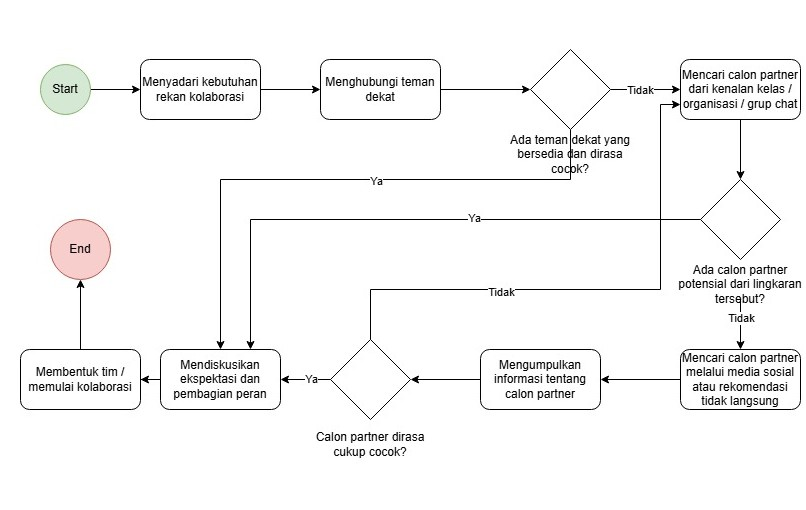
\includegraphics[width=0.7\textwidth]{image/41.jpg}
	\caption{\textit{Activity Diagram} Proses Pencarian Rekan Kolaborasi Mahasiswa Saat Ini}
	\label{gambar:41}
\end{figure}

Berdasarkan \textit{activity diagram} pada Gambar IV.1, dapat dilihat bahwa proses mahasiswa dalam mencari rekan kolaborasi saat ini masih berlangsung secara manual, tidak terstruktur, dan cenderung berulang. Mahasiswa biasanya memulai dengan mengidentifikasi kebutuhan kegiatan, kemudian mencoba menghubungi teman dekat atau kenalan yang mereka anggap potensial. Jika tidak ditemukan partner yang sesuai, mahasiswa melanjutkan pencarian melalui berbagai platform informal seperti grup percakapan, media sosial, atau rekomendasi dari teman lain.

Proses ini sangat bergantung pada jejaring sosial pribadi, sehingga sering kali menghasilkan kecocokan yang kurang optimal. Mahasiswa juga harus memeriksa kecocokan kandidat secara manual berdasarkan minat, \textit{skill}, pengalaman, dan gaya kerja, yang menyebabkan pencarian menjadi memakan waktu. Jika calon partner dianggap tidak sesuai, mahasiswa perlu mengulangi proses pencarian dari awal, menciptakan \textit{loop} yang tidak efisien. Hanya apabila ditemukan partner yang sesuai, proses dapat dilanjutkan ke tahap kesepakatan kolaborasi. Dengan demikian, \textit{behavioral model as-is} ini menunjukkan kebutuhan akan sistem rekomendasi yang lebih terstruktur untuk mempermudah dan mempercepat pencarian rekan kolaborasi.

\section{Model Sistem Usulan}
Model sistem usulan menggambarkan bagaimana proses pencarian rekan kolaborasi dapat dioptimalkan melalui sebuah platform terpusat yang menyediakan alur pencarian partner secara otomatis, terstruktur, dan berbasis rekomendasi. Berbeda dengan kondisi \textit{as-is} yang masih bergantung pada pencarian manual melalui berbagai platform informal—seperti grup percakapan, media sosial, atau jaringan pertemanan—dan sering kali membutuhkan banyak pengulangan proses untuk menemukan partner yang benar-benar sesuai, sistem \textit{to-be} dirancang untuk memberikan pengalaman pencarian yang lebih efisien dengan memanfaatkan data profil mahasiswa sebagai dasar pencocokan.

Pada model sistem usulan ini, proses rekomendasi \textit{People-to-People} dilakukan dengan memanfaatkan atribut profil mahasiswa seperti minat, keterampilan, pengalaman, gaya kerja, serta preferensi kontribusi. Informasi ini kemudian diproses menggunakan mekanisme \textit{Affinity-Based Matching} untuk menghasilkan daftar calon partner yang paling relevan bagi setiap pengguna. Dengan pendekatan ini, sistem tidak hanya mempersingkat waktu pencarian tetapi juga meningkatkan peluang terciptanya kolaborasi yang lebih produktif karena kecocokan partner dinilai melalui data yang lebih objektif.

Dalam penyajiannya, model sistem usulan diawali dengan \textit{behavioral model to-be} sebagai pembanding langsung dengan model \textit{as-is} yang sebelumnya sudah dijelaskan melalui \textit{activity diagram}. Pendekatan ini dilakukan untuk menekankan peningkatan signifikan pada alur proses setelah sistem baru diterapkan, sekaligus memperlihatkan bagaimana fitur rekomendasi menghilangkan hambatan-hambatan manual yang ada pada proses saat ini. Setelah alur \textit{to-be} dibahas, model dilanjutkan dengan \textit{context model} yang menggambarkan batas sistem dan pihak yang berinteraksi dengan platform, serta \textit{interaction model} atau \textit{use case diagram} untuk memperlihatkan hubungan antara pengguna dan fungsi-fungsi utama sistem.

\subsection{\textit{Behavioral Model To-Be}}
\textit{Behavioral model to-be} disajikan dalam bentuk \textit{activity diagram} mengikuti \textit{behavioral model as-is} yang telah dipaparkan sebelumnya. Diagram ini menggambarkan bagaimana alur pencarian rekan kolaborasi menjadi lebih efisien dan terstruktur setelah penggunaan modul rekomendasi \textit{People-to-People}. Model ini menekankan perbedaan antara proses manual yang terjadi saat ini dengan proses otomatis yang ditawarkan oleh sistem.
\begin{figure}[h] % pilihan opsi yang disarankan: t = top, b = bottom, h = here
	\centering
  \captionsetup{justification=centering}
    	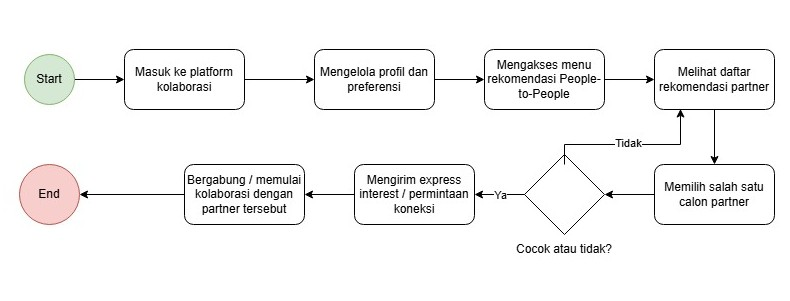
\includegraphics[width=0.7\textwidth]{image/42.jpg}
	\caption{\textit{Activity Diagram} Proses Pencarian Rekan Kolaborasi Mahasiswa Usulan}
	\label{gambar:42}
\end{figure}

\textit{Activity diagram} pada Gambar IV.2 menunjukkan bagaimana proses pencarian dan pemilihan rekan kolaborasi berubah secara signifikan pada sistem \textit{to-be} dibandingkan dengan kondisi \textit{as-is}. Pada sistem \textit{as-is}, mahasiswa harus mencari calon partner melalui berbagai platform informal, mengevaluasi kecocokan secara subjektif, serta mengulangi proses berkali-kali apabila calon partner tidak sesuai. Proses ini tidak efisien dan penuh ketidakpastian. Sebaliknya, pada model \textit{to-be}, sistem menyederhanakan seluruh proses melalui otomatisasi dan pemanfaatan data profil mahasiswa.

Proses dimulai ketika mahasiswa masuk ke platform dan memperbarui profil mereka, yang meliputi minat, keterampilan, pengalaman, gaya kerja, dan preferensi kontribusi. Informasi ini diproses oleh sistem untuk menghasilkan rekomendasi calon partner yang relevan melalui mekanisme \textit{Affinity-Based Matching}. Tidak seperti pada kondisi \textit{as-is}, mahasiswa tidak perlu lagi menebak kecocokan partner secara manual; sistem secara otomatis menyajikan daftar partner yang paling relevan berdasarkan pemodelan kecocokan yang terstruktur.

Ketika mahasiswa membuka detail calon partner yang direkomendasikan, mereka dapat langsung melihat atribut utama yang menjadi dasar kecocokan sehingga tidak perlu lagi melakukan analisis manual. Jika mahasiswa menyetujui rekomendasi tersebut, mereka dapat mengirim \textit{express interest} melalui platform untuk memulai kolaborasi. Dengan demikian, model \textit{to-be} tidak hanya mempercepat proses pencarian rekan kolaborasi, tetapi juga menghilangkan ketidakpastian, inkonsistensi, dan pengulangan yang umum terjadi pada proses \textit{as-is}.

\section{\textit{Context Model To-Be}}
Pada tahap ini dilakukan pemodelan konteks sistem untuk memberikan gambaran menyeluruh mengenai struktur solusi yang diusulkan serta hubungan antar elemen utamanya. Model yang digunakan pada tahap ini adalah \textit{context of system diagram}, yang berfungsi untuk menggambarkan batasan sistem, aktor yang terlibat, serta interaksi antara sistem dengan lingkungannya.
\begin{figure}[h] % pilihan opsi yang disarankan: t = top, b = bottom, h = here
	\centering
  \captionsetup{justification=centering}
    	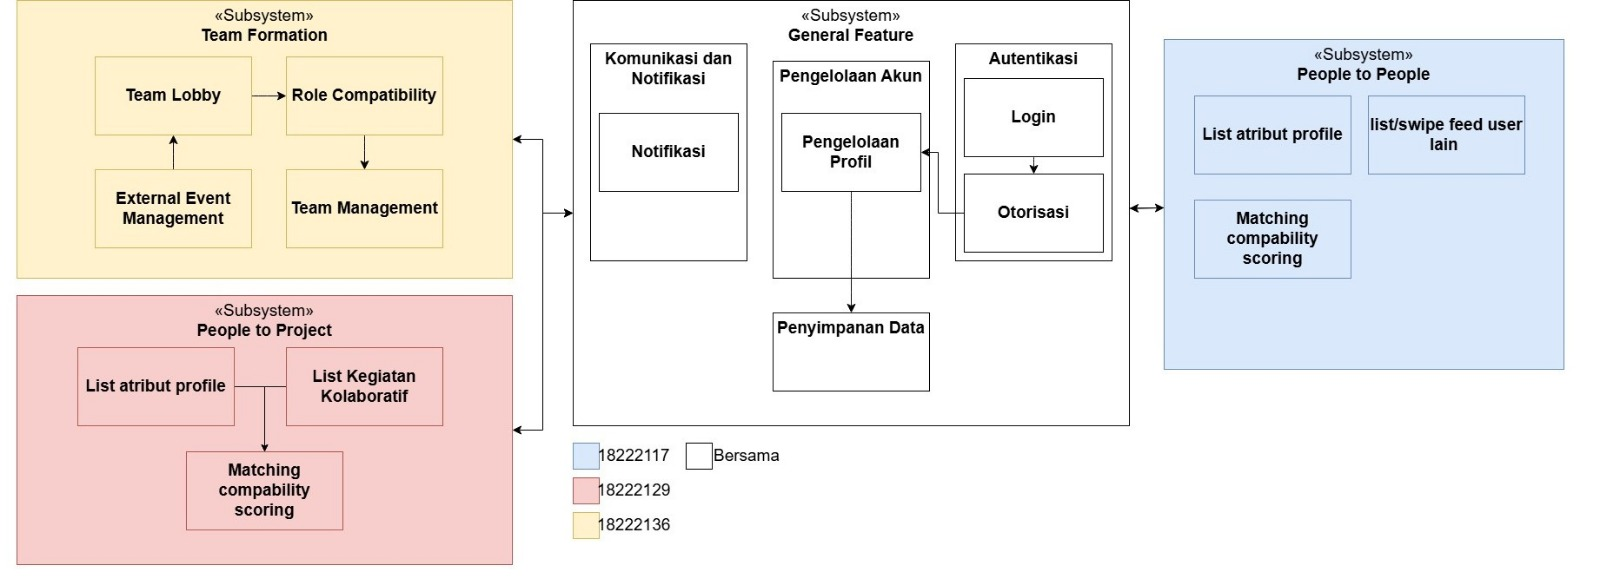
\includegraphics[width=0.7\textwidth]{image/43.jpg}
	\caption{\textit{Context of System Diagram}}
	\label{gambar:43}
\end{figure}

Berdasarkan Gambar IV.3, terlihat bahwa platform kolaborasi mahasiswa terdiri atas beberapa subsistem yang saling melengkapi, yaitu \textit{People to Project}, \textit{People to People}, \textit{Team Formation}, serta subsistem \textit{General Feature} yang menangani fungsi dasar seperti autentikasi, pengelolaan akun, dan penyimpanan data. Setiap subsistem memiliki peran, tanggung jawab, dan fungsi inti yang mendukung tujuan utama sistem, yaitu memfasilitasi proses pencarian kegiatan, pencarian partner, serta pembentukan tim secara terstruktur. Fitur rekomendasi yang dikembangkan dalam tugas akhir ini yaitu proses rekomendasi antara mahasiswa dengan calon rekan mahasiswa lainnya (\textit{People to People}).

\section{\textit{Interaction Model To-Be}}
Pada tahap \textit{interaction model}, sistem dimodelkan dari sudut pandang bagaimana pengguna berinteraksi dengan fungsi-fungsi yang disediakan oleh platform. Model yang digunakan adalah \textit{use case diagram}, karena model ini berperan sebagai jembatan antara kebutuhan fungsional hasil \textit{requirement engineering} dengan rancangan desain sistem yang akan diimplementasikan. \textit{Use case} memungkinkan perancang untuk mengidentifikasi siapa saja aktor yang terlibat dan bagaimana mereka memicu fungsi tertentu dalam sistem, sehingga setiap kebutuhan fungsional dapat dipastikan memiliki representasi operasional yang jelas.
\begin{longtable}{@{\extracolsep{\fill}} p{1.5cm} p{4cm} p{9cm}}
\caption{Kebutuhan Fungsional Sistem}\label{tbl:kebutuhan-fungsional} \\
\toprule
\textbf{Kode} & \textbf{Kebutuhan Fungsional} & \textbf{Deskripsi} \\
\midrule
\endfirsthead

\caption[]{Kebutuhan Fungsional Sistem (lanjutan)} \\
\toprule
\textbf{Kode} & \textbf{Kebutuhan Fungsional} & \textbf{Deskripsi} \\
\midrule
\endhead

\midrule
\multicolumn{3}{r}{\textit{Bersambung ke halaman berikutnya}} \\
\bottomrule
\endfoot

\bottomrule
\endlastfoot

% ========= F01 =========
F01 & Pengelolaan profil pengguna &
Sistem harus mampu mengumpulkan, menyimpan, dan memperbarui data profil mahasiswa, termasuk minat, keterampilan, pengalaman proyek, gaya kerja, preferensi kontribusi, dan ketersediaan waktu. Data ini digunakan sebagai dasar utama dalam proses rekomendasi. \\

% ========= F02 =========
F02 & Pembaruan preferensi pengguna &
Pengguna harus dapat memperbarui preferensi kolaborasi sewaktu-waktu agar sistem dapat menghasilkan rekomendasi partner yang tetap relevan dengan kondisi terbaru pengguna. \\

% ========= F03 =========
F03 & Pengelolaan data atribut kecocokan &
Sistem harus menyediakan struktur data terstandardisasi untuk menyimpan atribut yang digunakan dalam penilaian kesesuaian antar pengguna, seperti minat, \textit{skill}, \textit{tools/tech stack}, pengalaman, motivasi, serta gaya kerja. Seluruh atribut harus dapat diakses oleh \textit{engine} pencocokan. \\

% ========= F04 =========
F04 & Mekanisme pencocokan (\textit{Affinity-Based Matching}) &
Sistem harus memiliki mekanisme untuk menghitung skor kecocokan antar pengguna menggunakan metode \textit{Affinity-Based Matching} dengan mempertimbangkan bobot atribut yang relevan. Mekanisme ini menjadi inti fitur rekomendasi. \\

% ========= F05 =========
F05 & Penyajian hasil pencocokan &
Sistem harus dapat menampilkan daftar calon partner dalam bentuk \textit{feed} rekomendasi yang diurutkan berdasarkan tingkat kecocokan tertinggi dari hasil perhitungan \textit{affinity}. \\

% ========= F06 =========
F06 & Tampilan detail profil calon partner &
Sistem harus menyediakan tampilan profil lengkap calon partner yang menampilkan atribut penting secara terstruktur, sehingga pengguna dapat memahami alasan dan dasar kecocokan dari rekomendasi tersebut. \\

% ========= F07 =========
F07 & Interaksi dasar antar pengguna &
Sistem harus menyediakan fitur interaksi dasar seperti \textit{save profile}, \textit{express interest}, dan \textit{connect request} untuk memungkinkan pengguna menindaklanjuti rekomendasi dan memulai kolaborasi. \\

\end{longtable}

Dalam konteks subsistem \textit{People-to-People Recommendation}, kebutuhan fungsional yang telah dirumuskan pada Bab III diturunkan ke dalam serangkaian \textit{use case} seperti pada Tabel IV.1 yang menggambarkan alur interaksi mahasiswa sebagai pengguna utama terhadap sistem rekomendasi partner kolaborasi. Setiap \textit{use case} memetakan tindakan pengguna terhadap sistem, keluaran yang diharapkan, serta batasan-batasan yang terkait dengan proses pencocokan partner. Dengan demikian, \textit{interaction model} tidak hanya memastikan bahwa sistem mendukung kebutuhan pengguna, tetapi juga menyediakan dasar yang kuat untuk pemodelan perilaku dan implementasi prototipe pada tahap berikutnya.
\begin{figure}[h] % pilihan opsi yang disarankan: t = top, b = bottom, h = here
	\centering
  \captionsetup{justification=centering}
    	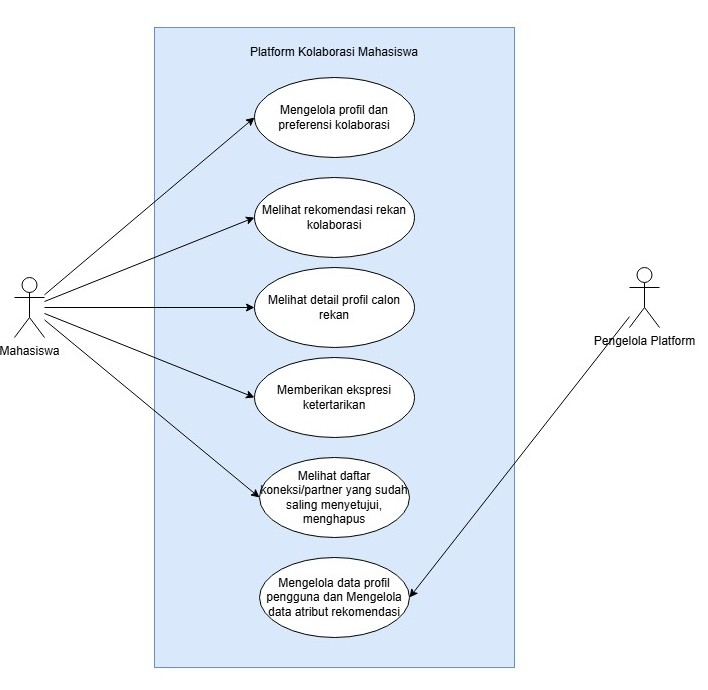
\includegraphics[width=0.7\textwidth]{image/44.jpg}
	\caption{\textit{Use Case Diagram} Modul \textit{People-to-People Recommendation}}
	\label{gambar:44}
\end{figure}

Diagram \textit{use case} pada Gambar IV.4 memperlihatkan interaksi antara aktor Mahasiswa dengan fungsi inti yang disediakan oleh modul \textit{People-to-People Recommendation}. Mahasiswa sebagai aktor utama berinteraksi dengan enam \textit{use case}, yaitu mengelola profil pengguna, melihat rekomendasi rekan kolaborasi, melihat detail profil calon partner, melakukan penyaringan rekomendasi, memberikan \textit{express interest}, dan mengelola koneksi kolaborasi. Keenam \textit{use case} tersebut mewakili seluruh alur penggunaan sistem dari sudut pandang mahasiswa, mulai dari pengisian profil hingga menerima rekomendasi partner yang relevan berdasarkan hasil pencocokan otomatis.

Sementara itu, aktor Pengelola Platform berperan dalam mengelola data umum yang menjadi dasar sistem, seperti verifikasi data profil dan pemeliharaan atribut yang digunakan dalam mekanisme rekomendasi. Namun pada tugas akhir ini, peran Admin dapat disederhanakan karena fokus pengembangan berada pada proses pencocokan mahasiswa dan interaksinya terhadap modul rekomendasi.